\section{Visualization Design}
\label{sec:solution:viz}

Each of the six themes cataloged in Section~\ref{sec:solution:themes}
requires several visualizations to address the analytical question
that defines it. The selection of a primitive chart type for each
visualization is constrained by the Chart Selection Rubric of
Section~\ref{sec:foundations:primitives:rubric} and by the storytelling
invariants of Section~\ref{sec:solution:interaction:storytelling}. The
catalog resolves to \textbf{twenty canvases across the six themes
(4+4+3+4+2+3)}, with three further design decisions shaping its shape:
within-theme ordering by persona breadth (charts that serve all three
personas appear first; specialist charts appear last); a click-to-entity-detail
panel as the system's Connect realization (every chart's primary click
opens the panel of Section~\ref{sec:solution:interaction:detail},
following the Yi (2007) seven-category interaction
taxonomy~\cite{yi2007interaction}); and per-chart implementation
availability tracked against the data inventory of
Section~\ref{sec:solution:dataset} through a four-tier feasibility
audit. The per-theme selection itself --- each theme's canvases, the
primitive chosen for each, and the defense against the obvious
alternatives --- is recorded in Appendix~E, alongside the methodology
side-panel design and the primitives that were considered and rejected.

Two charts in the catalog carry visible data caveats. Chart 3.2
Bus$\leftrightarrow$Metro Sankey (indicative) uses a hard-coded
Metro Line 1 schedule fallback because the Metro arrival schedule is
not in the published dataset; the qualifier ``indicative'' is part of
the chart's title. Chart 4.4 is reframed from the original
``Promotion DiD'' framing to a ``Free-fare student-day lift
waterfall'' because the \texttt{promotion\_code} field is 99\% null in
\texttt{afc.payments}; the free-pass fare class (9\% of boardings) is
populated in \texttt{afc.tickets.fare\_class} and serves as the proxy
intervention event. Both caveats are exposed in the chart's
Methodology Side-Panel (Appendix~E).

Table~\ref{tab:viz:traceability} records the requirements traceability
across the three layers: each of the fourteen stakeholder questions
from Section~\ref{sec:solution:problem:questions} is matched to the
themes that answer it. The matrix surfaces both the coverage claim
(every question reaches at least one theme) and the cross-theme
dependencies (several questions admit answers from more than one
theme).

\begin{table}[!htbp]
\centering
\caption{Stakeholder questions mapped to themes (tick = addressed).}
\label{tab:viz:traceability}
\footnotesize
\renewcommand{\arraystretch}{1.2}
\begin{tabularx}{\linewidth}{p{0.9cm} X c c c c c c}
\hline
\textbf{Q.} & \textbf{Question} & \rotatebox{60}{\textbf{School}} & \rotatebox{60}{\textbf{Demand}} & \rotatebox{60}{\textbf{Spatial}} & \rotatebox{60}{\textbf{Financial}} & \rotatebox{60}{\textbf{Network}} & \rotatebox{60}{\textbf{Routes}} \\
\hline
P-Q1 & Is route X reliable enough to commit to?               &     & $\checkmark$ &     &     &     & $\checkmark$ \\
P-Q2 & When is route X / stop Y least crowded?                &     & $\checkmark$ & $\checkmark$ &     &     &     \\
P-Q3 & Does this route serve my school's commute window?      & $\checkmark$ &     &     &     &     &     \\
C-Q1 & Which routes are over- or under-supplied vs demand?    &     & $\checkmark$ &     & $\checkmark$ &     &     \\
C-Q2 & Route-level revenue picture (\textdong/trip, ghost-run \%)? &     &     &     & $\checkmark$ &     &     \\
C-Q3 & How do I rank vs other operators on the same corridor? &     &     &     & $\checkmark$ &     &     \\
C-Q4 & Did my last promotion lift ridership?                  &     &     &     & $\checkmark$ &     &     \\
A-Q1 & Where does supply diverge from demand network-wide?    &     & $\checkmark$ & $\checkmark$ &     & $\checkmark$ &     \\
A-Q2 & Which routes have QoS-1/2/3 reliability problems?      &     &     &     &     & $\checkmark$ & $\checkmark$ \\
A-Q3 & How does the network absorb and recover from shocks?   &     &     &     &     & $\checkmark$ &     \\
A-Q4 & Where are coverage and equity gaps (schools, wards)?   & $\checkmark$ &     & $\checkmark$ &     &     &     \\
A-Q5 & How well does bus integrate with Metro Line~1?         &     &     & $\checkmark$ &     &     &     \\
A-Q6 & What is the operator-concentration market structure?   &     &     &     & $\checkmark$ &     &     \\
A-Q7 & 14-day demand forecast per route?                      &     & $\checkmark$ &     &     &     &     \\
\hline
\textbf{Canvases} & \multicolumn{1}{r}{\textbf{per theme}}    & \textbf{4} & \textbf{4} & \textbf{3} & \textbf{4} & \textbf{2} & \textbf{3} \\
\hline
\end{tabularx}
\end{table}

Figure~\ref{fig:solution:viz_catalogue_map} summarizes the full
catalog as a six-column map, with each canvas ordered top-to-bottom
by persona breadth within its theme column. Two canvases carry a
visible caveat marker: chart~3.2 (indicative Metro schedule) and
chart~4.4 (free-fare reframe). The per-theme selection and rationale
behind each canvas are developed in Appendix~E.

\begin{figure}[!htbp]
\centering
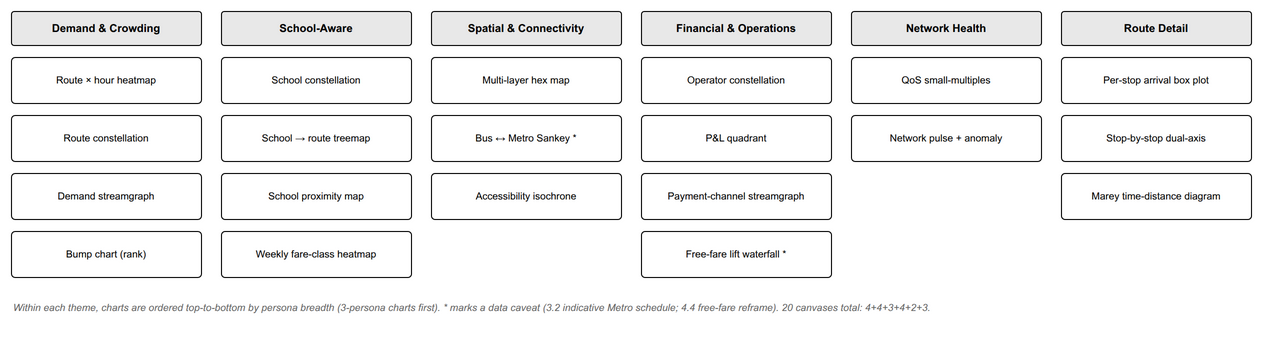
\includegraphics[width=0.98\linewidth]{images/diagrams/solution_catalogue_map.png}
\caption{Catalog map: twenty canvases across six themes (4+4+3+4+2+3), ordered by persona breadth within each theme.}
\label{fig:solution:viz_catalogue_map}
\end{figure}
